% Please do not change the document class
\documentclass{scrartcl}

% Please do not change these packages
\usepackage[hidelinks]{hyperref}
\usepackage[none]{hyphenat}
\usepackage{setspace}
\usepackage{graphicx}
\doublespace

% You may add additional packages here
\usepackage{amsmath}

% Please include a clear, concise, and descriptive title
\title{How can game developers accomodate for people with hard of hearing?}

% Please do not change the subtitle
\subtitle{COMP160 - Software Engineering Essay}

% Please put your student number in the author field
\author{1601002}

\begin{document}

\maketitle

\abstract
The gaming industry attracts more and more people everyday with special needs, so the game developers need to compensate for the ever increasing numbers of the diverse audience it caters to, this paper aims to address the issues a person with a hearing impairment may face when gaming and bring them to light. The industry has been successful in appealing to fans of the sports genre and education to help the academically challenged people with 'wii sports' and 'brain age' respectively. So which games already help the hard of hearing and what can game developers learn from these games?

\section{Introduction}
The demand for software which is accessible by members of the public suffering with mental and physical impairments has been on the rise and since June 2001 under section 508 of the Rehabilitation act \cite{cohen2005accessibility} agencies in America have been obliged to offer aids to the people to allow them to access information which others are also able to access. Over one in five adults suffer from some sort of disability, both mental and physical, worldwide \cite{sierkowski2002achieving} which would mean ignoring this issue would effectively be discarding 20 percent of the potential market which for any reasonable developer is too big a margin to ignore.  Another issue which doesn't help the matter is that individuals do not know what the game includes, in terms of accessibility, through no fault of their own this is due to the simple fact that game cases do not display the accessibility features anywhere on it. \cite {bierre2005game}. Due to the neglect made towards gamers with disabilities over the years the games industry has grown apathetic and as a result the games being produced have not been adequately influenced by accessibility standards.\cite{porter2013empirical}

\section{Pre-existing accessibility}
Accessibility features can either be gameplay changes which then require the structure of the software to be altered, or vice versa. An example of where the code and underlying mechanics of the game is built around the accessibility of the gameplay is if the visuals of the game were to alter based on the audio side of the game. This can be seen in games where music dictates the gameplay, examples are: Beat Hazard\cite {game:beathazard}, Symphony\cite {game:symphony} and Audio Surf\cite {game:audiosurf}. Since studies show that deaf people can 'feel' noises \cite {Nanayakkara} why shouldn't it be possible for deaf people to interpret noise from visual stimuli, which some game developers are already testing on children to improve their timing  \cite {Jouhtimaki}. In addition to this, there has been research into whether comprehensive testing for younger children with hearing difficulties could be scrapped in favour of alternative examination methods \cite{Mich} this could pave the way for a a brand new market being opened in the gaming industry specifically for children in education who suffer from hearing difficulties. Sega's 1976 Moto-Cross was the first comercial video game to incorporate haptic feedback into their game play, where when a vehicle collided with another object the handlebars would vibrate \cite {Sega}. 

 Another study made around people with hearing impairments took 111 participants, 61 percent of which play or have ever played games\cite {Coutinho} The study showed that when asked about their favourite and least favourite games, most of the participants stated they enjoyed simple puzzle games with limited reading and learning involved, whilst their least favourite game genres were First Person Shooters (FPS) and Role Playing Games (RPG) as both require quick reactions or heavy reading \cite {Coutinho}. Some games already have features which cater to the hard of hearing by including sign language which the individuals would find familiar \cite{Bouzid}. This could convey information about the game, such as what is happening in the game at that moment or what a character is saying in a dialogue or perhaps even how they are saying it. However in most cases this option could be made obsolete by simple subtitles.

\section{Structural accessibility}
All accessibility features of games required a line of code for them to operate, in this section I will be covering how different features are designed for deaf people.
Typically the first port of call for a deaf or hard of hearing individual viewing anything is to try and turn the subtitles on which produces a line of words at the bottom center of the screen in the game window. For this to occur there first needs to be a script for the whole game which can be called by a function in the code. Moreover, companies such as Electronic Arts and Ubisoft tend to develop AAA games (games with generally high economic expenses), who would generally avoid developing games from scratch aimed at people with disabilities due to time, coding and money. Research into game developers in Panama revealed that a majority of game developers do not interact with their target audience when developing an accessible game for a particular disability. \cite {moreno}. Other attempts to include people who are deaf with more than just gaming is a study conducted by Jones, Bench and Ferons who looked into using a HMD (Head mounted display) as an augmented tool for deaf children to read and interpret words by taking pictures of words that the child was pointing at \cite {Jones}.
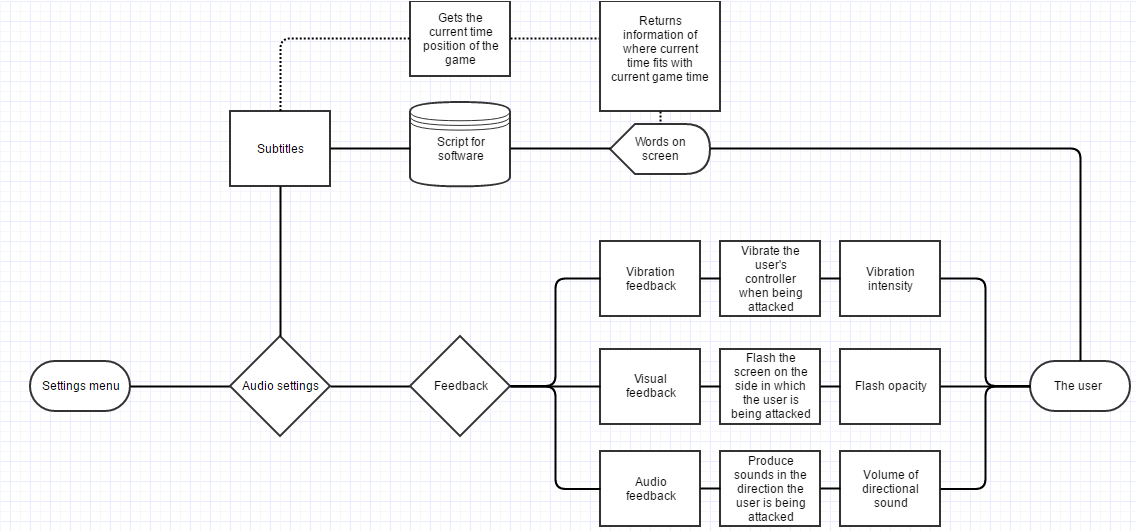
\includegraphics [scale=0.5]{gliffy}

\section{Conclusion}
After examining each research article it would appear that game developers can accommodate for people with hard of hearing, among other conditions, the only reason they do not is due to
financial and/or time restrictions. However there are some games, such as Beat Hazard, which are designed in such a way which, whether intentional or not provide potential accessibility to people with hearing difficulties. Whereas the more popular and developed games seem to contain less accessible means for a disabled person to play their game, the accessibility features offered by these games are usually quite simple, such as closed captions or flashes of red to indicate the direction in which the character is being attacked from.

\bibliographystyle{ieeetran}
\bibliography{references}


\end{document}
